\documentclass{standalone}
\usepackage{pgfplots}

\pgfplotsset{compat=1.16,width=16cm}

\begin{document}
	
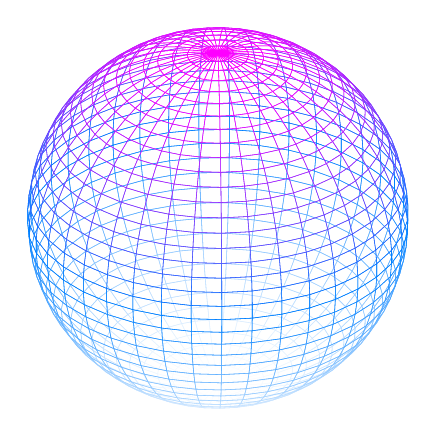
\begin{tikzpicture}
	\begin{axis}[
		hide axis,
		axis equal image,
		view={135}{30}, % Adjust the view angle to give a better 3D effect
		colormap/cool,
		]
		\addplot3[
		very thin,
		mesh,
		samples=40, % Adjust the number of samples if needed for smoothness or performance
		domain=0:360,
		y domain=0:180,
		] 
		(
		{sin(y)*cos(x)}, % x = sin(theta)*cos(phi)
		{sin(y)*sin(x)}, % y = sin(theta)*sin(phi)
		{cos(y)}         % z = cos(theta)
		);
	\end{axis}
\end{tikzpicture}
	
\end{document}
